% Praeambel
\documentclass{report}

  % verwendete Packages
\usepackage[utf8]{inputenc}
\usepackage{graphicx}
\usepackage[english, german]{babel}
\usepackage{listings}
\usepackage{xcolor}
\usepackage{moreverb}
\usepackage{minted}

\graphicspath{ {images/} } % sage Latex, dass es die Bilder unter dem Ordner 'images' im aktuellen Ordner findet!
\lstset { %
    language=C++,
    backgroundcolor=\color{black!5}, % set backgroundcolor
    basicstyle=\footnotesize,% basic font setting
} % fuer C++ anzeigen

  % Titel-Einstellungen
\title{Code Dokumentation - Wissenschaftliches Programmieren für Ingenieure im Wintersemester 2018/2019}
\author{Jens Weber - Matrikel Nummer: 1851194}
\date{18.12.2018}


% Dokument
\begin{document}

\maketitle{}
\clearpage{}


\tableofcontents{}
\clearpage{}

\chapter{Aufgabe 1: Rechnen mit komplexen Zahlen}

\section{Verwendung des Codes}\label{sec:verwendungA1}

Der für diese Aufgabe verwendete Code ist in \ref{sec:codeA1} zu finden. Er lässt sich mit dem Makefile kompilieren.
Nach dem das kompilieren erfolgreich abgeschlossen ist, startet man das Programm mit:
\begin{lstlisting}[language=bash]
  $ ./aufgabe_1
\end{lstlisting}
Die Berechnungsergebnisse werden im Terminal ausgegeben.



\section{Ergebnisse der Berechnung}\label{sec:ergebnisseA1}
Hier sind die Ergebnisse der Berechnung (\textbf{Aufgabenteil A)}), ausgehend von:

\begin{equation}\label{eq:gegZ1}
  z_1 = 2 + 7*i
\end{equation}
\begin{equation}\label{eq:gegZ2}
  z_2 = 42 - 9*i
\end{equation}
\begin{equation}\label{eq:gegZ3}
  z_3 = -11 + 19*i
\end{equation}


, tabellarisch in \ref{tab:resA1} aufgeführt.
\bigskip % platz bis zur naechsten Zeile lassen!

\begin{center}
\begin{tabular}{c|c}\label{tab:resA1}
Formel & Ergebnis \\
\cline{1-2}
$z_4 = z_1 * z_2$ & $147 + 276*i$ \\
\cline{1-2}
$z_5 = (z_1 + z_2)$ & $44 - 2*i$ \\
\cline{1-2}
$z_6 = (z_1 + z_2)*2$ & $88 - 4*i$  \\
\cline{1-2}
$z_7 = (z_2 + z_3)*z_1$ & $-8 + 237*i$ \\
\cline{1-2}
$z_8 = z_1 + 5$ & $7 + 7*i$ \\
\cline{1-2}
$z_9 = -z_1 + z_2$ & $40 - 16*i$ \\
\cline{1-2}
\end{tabular}
\label{table:resA1}
\end{center}


\subsection{Code in Operatorschreibweise}

Entsprechend \testbf{Aufgabenteil B} wird hier der Code zur Berechnung der Ergebnisse in Operatorschreibweise als Quellcode aufgelistet. \\
Eine ausführbares Programm findet sich im Ordner \textit{aufgabe\_1} mit dem Namen \textit{main\_complex\_operator\_schreibweise.cpp}


\begin{lstlisting}
z4.operator=(z1.operator*(z2));
z5.operator=((z1.operator+(z2)));
z6.operator=((z1.operator+(z2)).operator*(2.));
z7.operator=((z2.operator+(z3)).operator*(z1));
z8.operator=(z1.operator+(5.));
z9.operator=(z1.operator-().operator+(z2));
\end{lstlisting}



\section{Code}\label{sec:codeA1}

Im Folgenden ist der komplette Code, inklusive Makefile zu Aufgabe 1 zu finden.

\textbf{complex.h: }
\inputminted[autogobble]{C++}{complex_a1.h}

\clearpage{}
\textbf{complex.cpp: }
\inputminted[autogobble]{C++}{complex_a1.cpp}

\clearpage{}
\textbf{main\_complex\_beispiel.cpp: }
\inputminted[autogobble]{C++}{main_complex_beispiel_a1.cpp}

\clearpage{}
\textbf{Makefile: }
\inputminted[autogobble]{make}{Makefile_a1}


\chapter{Aufgabe 2: Untersuchung der Konvergenz komplexer Zahlenfolgen}

\section{Verwendung des Codes}\label{sec:verwendungA2}
Der Code in Ordner \textit{aufgabe\_2} lässt sich mit dem enthaltenen Makefile bauen.
Das entstandene Programm lässt sich auf drei Arten starten:

\begin{enumerate}
  \item Direkte Nutzereingabe der auszuwertenden Parameter
  \item Übergabe der gegebenen Start-Dateien mittels des Operators \textit{<} .
  \item Mittels des angefügten Shell-Skripts (\textit{run\_all.sh}), welches in \ref{sec:codeA2} zu finden ist.
\end{enumerate}

Nachdem die Berechnungen abgeschlossen sind, können die Ergebnisbilder mit dem ebenfalls in \ref{sec:codeA2} angefügten Gnuplot-Skript erstellt werden. \\
Dafür wird Gnuplot aufgerufen:

\begin{lstlisting}[language=bash]
  $ gnuplot
\end{lstlisting}

Und anschließend das Skript zum erstellen der Ergebnisbilder aufgerufen:

\begin{lstlisting}[language=bash]
  > load 'plot_result.gp'
\end{lstlisting}

Die Resultate befinden sich nun im Ordner \textit{aufgabe\_2}.

\section{Ergebnisse der Konvergenzanalyse}\label{sec:ergebnisseA2}
Die Ergebnisse der Konvergenzanalyse mit allen Datensätzen ist im Folgenden aufgeführt:

\clearpage{}
\textbf{start1A.dat:}

\begin{center}
\begin{tabular}{c|c}
Iterationsvorschrift & $1$ \\
\cline{1-2}
Wertebereich & $(-1.5, -1) - (1.5, 1)$ \\
\cline{1-2}
Unterteilung (Nxmax, Nymax) & $750, 500$ \\
\cline{1-2}
Exponent & $2$  \\
\cline{1-2}
Nmax & $2000$ \\
\cline{1-2}
Rc & $100$ \\
\cline{1-2}
Komplexe Konstante c0 & $(-0.75, 0.1)$ \\
\cline{1-2}
\end{tabular}
\label{tab:resA2_1}
\end{center}

\begin{figure}[h]
    \centering
    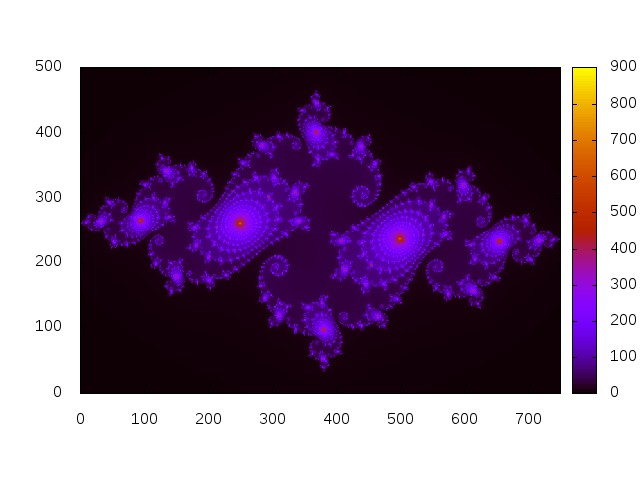
\includegraphics[scale=0.7]{ergebnis1A}
    \caption{Ergebnis des Datensatz 1A}
    \label{fig:ergebnis1A} % ID um zu referenzieren mit \ref{fig:ergebnis1A}
\end{figure}

\clearpage{}
\textbf{start1B.dat:}

\begin{center}
\begin{tabular}{c|c}
Iterationsvorschrift & $1$ \\
\cline{1-2}
Wertebereich & $(-1.5, -1) - (1.5, 1)$ \\
\cline{1-2}
Unterteilung (Nxmax, Nymax) & $750, 500$ \\
\cline{1-2}
Exponent & $2$  \\
\cline{1-2}
Nmax & $2000$ \\
\cline{1-2}
Rc & $100$ \\
\cline{1-2}
Komplexe Konstante c0 & $(-0.75, 0.55)$ \\
\cline{1-2}
\end{tabular}
\label{tab:resA2_2}
\end{center}

\begin{figure}[h]
    %\centering
    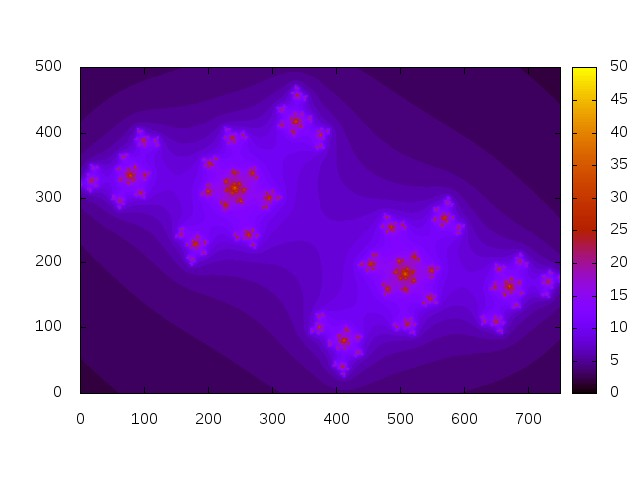
\includegraphics[scale=0.7]{ergebnis1B}
    \caption{Ergebnis des Datensatz 1B}
    \label{fig:ergebnis1B} % ID um zu referenzieren mit \ref{fig:ergebnis1A}
\end{figure}


\clearpage{}
\textbf{start2A.dat:}

\begin{center}
\begin{tabular}{c|c}
Iterationsvorschrift & $2$ \\
\cline{1-2}
Wertebereich & $(-2, -1) - (1, 1)$ \\
\cline{1-2}
Unterteilung (Nxmax, Nymax) & $750, 500$ \\
\cline{1-2}
Exponent & $2$  \\
\cline{1-2}
Nmax & $200$ \\
\cline{1-2}
Rc & $2$ \\
\cline{1-2}
Komplexe Konstante c0 & $(0, 0)$ \\
\cline{1-2}
\end{tabular}
\label{tab:resA2_3}
\end{center}

\begin{figure}[h]
    %\centering
    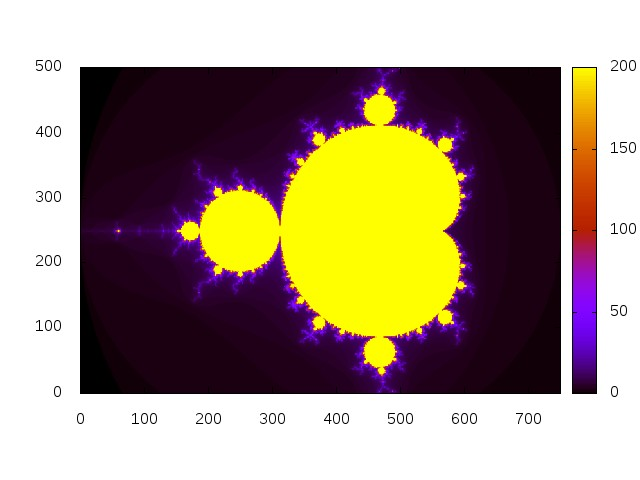
\includegraphics[scale=0.7]{ergebnis2A}
    \caption{Ergebnis des Datensatz 2A}
    \label{fig:ergebnis2A} % ID um zu referenzieren mit \ref{fig:ergebnis1A}
\end{figure}

\clearpage{}
\textbf{start2B.dat:}

\begin{center}
\begin{tabular}{c|c}
Iterationsvorschrift & $2$ \\
\cline{1-2}
Wertebereich & $(-1.5, 1) - (0, 0)$ \\
\cline{1-2}
Unterteilung (Nxmax, Nymax) & $750, 500$ \\
\cline{1-2}
Exponent & $2$  \\
\cline{1-2}
Nmax & $200$ \\
\cline{1-2}
Rc & $2$ \\
\cline{1-2}
Komplexe Konstante c0 & $(0, 0)$ \\
\cline{1-2}
\end{tabular}
\label{tab:resA2_4}
\end{center}

\begin{figure}[h]
    %\centering
    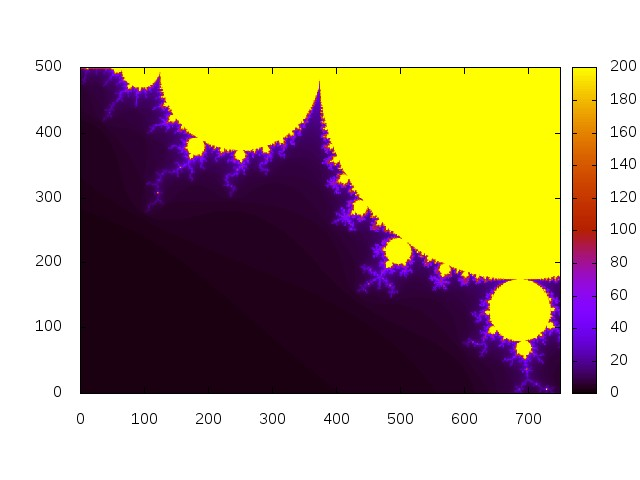
\includegraphics[scale=0.7]{ergebnis2B}
    \caption{Ergebnis des Datensatz 2B}
    \label{fig:ergebnis2B} % ID um zu referenzieren mit \ref{fig:ergebnis1A}
\end{figure}


\clearpage{}
\textbf{start3A.dat:}

\begin{center}
\begin{tabular}{c|c}
Iterationsvorschrift & $3$ \\
\cline{1-2}
Wertebereich & $(-1.5, -1) - (1.5, 1)$ \\
\cline{1-2}
Unterteilung (Nxmax, Nymax) & $750, 500$ \\
\cline{1-2}
Exponent & $4$  \\
\cline{1-2}
Nmax & $2000$ \\
\cline{1-2}
Rc & $200$ \\
\cline{1-2}
Komplexe Konstante c0 & $(0, 0)$ \\
\cline{1-2}
\end{tabular}
\label{tab:resA2_5}
\end{center}

\begin{figure}[h]
    %\centering
    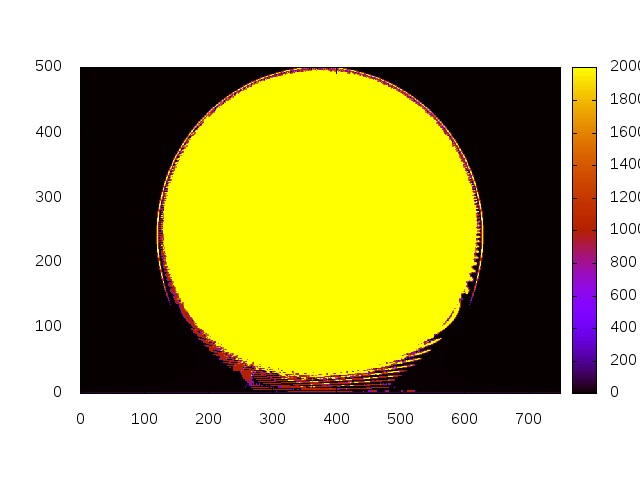
\includegraphics[scale=0.7]{ergebnis3A}
    \caption{Ergebnis des Datensatz 3A}
    \label{fig:ergebnis3A} % ID um zu referenzieren mit \ref{fig:ergebnis1A}
\end{figure}


\section{Code}\label{sec:codeA2}

Hier wird der Code für Aufgabe 2, inklusiver des Makefiles und der Shell, bzw Gnuplot Skripte aufgeführt: \\
\\

\textbf{complex.h: }
\inputminted[autogobble]{C++}{complex_a2.h}

\clearpage{}
\textbf{complex.cpp: }
\inputminted[autogobble]{C++}{complex_a2.cpp}

\clearpage{}
\textbf{main\_convergenz.cpp: }
\inputminted[autogobble]{C++}{main_convergenz_a2.cpp}

\clearpage{}
\textbf{Makefile: }
\inputminted[autogobble]{make}{Makefile_a2}

\clearpage{}
\textbf{Shell Skript: }
\inputminted[autogobble]{bash}{run_all_a2.sh}


\clearpage
\textbf{plot\_result.gp: }
\begin{lstlisting}
set pm3d map

do for [ii=1:3:1] {
  file=sprintf('ergebnis%dA.dat',ii)

  resultName=sprintf('ergebnis%dA.jpg',ii)
  set term jpeg
  set output resultName

  set xrange[0:750]
  set yrange[0:500]

  splot file u ($1):($2):($3)

  if (ii < 3) {
    file=sprintf('ergebnis%dB.dat',ii)

    resultName=sprintf('ergebnis%dB.jpg',ii)
    set term jpeg
    set output resultName

    splot file u ($1):($2):($3)
  }
}
\end{lstlisting}


\end{document}
